\documentclass{beamer}
\usepackage{graphicx} % To include images (e.g., QR codes)
\usepackage{hyperref} % To add clickable hyperlinks
\usepackage{xcolor}   % For defining custom colors
\usepackage{iexec} % For running shell commands to get the Git commit hash (document version)
\newcommand{\gitAbbrevHash}{\iexec{git rev-parse --short HEAD}} % Create a new command to retrieve the abbreviated Git commit hash
%\usepackage{fontspec} % Uncomment this line if using LuaLaTeX or XeLaTeX for custom fonts

% -----------------------------------------------------------------------------
% Hyperlink Colors Configuration
% Define the colors for links in the document
% -----------------------------------------------------------------------------
\hypersetup{
    colorlinks=true,   % Enable colored links instead of boxed links
    linkcolor=blue,    % Color for internal document links (e.g., TOC links)
    urlcolor=cyan      % Color for external links (e.g., URLs)
}

% -----------------------------------------------------------------------------
% Footer Configuration
% Customizes the footer layout, including the document version and page number
% -----------------------------------------------------------------------------
\setbeamertemplate{footline}{%
  \leavevmode%
  \hbox{
    % Left: Organization Name
    \begin{beamercolorbox}[wd=.35\paperwidth,ht=2.25ex,dp=1ex,leftskip=.3cm]{author in head/foot}%
      Wireless Club at Northeastern University%
    \end{beamercolorbox}%
    % Center: Workshop Name
    \begin{beamercolorbox}[wd=.20\paperwidth,ht=2.25ex,dp=1ex,center]{author in head/foot}%
      Yagi Antenna Workshop%
    \end{beamercolorbox}%
    % Center: Semester Information
    \begin{beamercolorbox}[wd=.15\paperwidth,ht=2.25ex,dp=1ex,center]{author in head/foot}%
      Fall 2024%
    \end{beamercolorbox}%
    % Right: Version (Git commit hash) and Page Number
    \begin{beamercolorbox}[wd=.30\paperwidth,ht=2.25ex,dp=1ex,rightskip=.3cm plus1fil]{author in head/foot}%
      Version: \gitAbbrevHash{} \hspace{1em} \insertframenumber/\inserttotalframenumber%
    \end{beamercolorbox}}%
  \vskip0pt%
}

% -----------------------------------------------------------------------------
% Document Information (Title Page)
% -----------------------------------------------------------------------------
\title{Yagi Antenna Workshop}
\subtitle{Building a Tape Measure Antenna}
\author{Northeastern University Wireless Club - W1KBN}
\date{September 9, 2024}

\begin{document}

% -----------------------------------------------------------------------------
% Slide: Title with QR Code for Sign-In
% This slide contains the title of the workshop and a QR code for participants to sign in
% -----------------------------------------------------------------------------
\begin{frame}
    \titlepage % Displays the title, subtitle, author, and date
    \vspace{-1cm} % Adjusts vertical spacing to make room for the QR code
    \begin{center}
        \textbf{Sign in here!} \\ % Text prompt for the sign-in
        
\includegraphics[width=0.30\textwidth]{images/qrcode.png} % QR code image for sign-in
        \vspace{-0.3cm} % Adjust spacing between text and QR code
        \\
        {\small \url{https://l.w1kbn.org/signin}} % Sign-in URL displayed below the QR code
    \end{center}
\end{frame}

% -----------------------------------------------------------------------------
% Slide: Welcome Introduction
% An introduction slide welcoming attendees and providing an overview of the workshop
% -----------------------------------------------------------------------------
\begin{frame}
    \frametitle{Welcome to Our First Workshop!}
    \begin{itemize}
        \item Welcome to the Wireless Club's first workshop of the semester!
        \item Who we are:
        \begin{itemize}
            \item We are Northeastern University's Wireless Club, passionate about electronics, antennas, and wireless technologies.
            \item Our workshops are designed to be beginner-friendly, so all skill levels are welcome.
        \end{itemize}
        \item Today’s Plan:
        \begin{itemize}
            \item Introduction to HAM Radio and Antennas
            \item Step-by-step Yagi Antenna build using a tape measure and basic materials
            \item Q&A and hands-on assembly
        \end{itemize}
        \item Visit our website for more information: \url{https://nuwireless.org/}
    \end{itemize}
\end{frame}

% -----------------------------------------------------------------------------
% Slide: General Information and Sign-In
% -----------------------------------------------------------------------------
\begin{frame}
    \frametitle{Welcome!}
    \begin{itemize}
        \item Wireless Club Meetings: Thursdays at 7 PM @ 503 Hayden (with free pizza!)
        \item Workshop Meetings: Mondays at 7 PM @ East Village, Room 010
        \item Join our Slack: \url{https://neuwireless.slack.com/join/signup}
        \item Join our mailing list: \url{http://eepurl.com/gduCIr}
        \item Scope of today's workshop:
        \begin{itemize}
            \item Quick Introduction to HAM Radio
            \item Basics of Antennas
            \item Hands-on Build: \url{https://www.instructables.com/The-Tape-Measure-Antenna/}
        \end{itemize}
        \item Don’t forget to sign in: \url{https://l.w1kbn.org/signin}
    \end{itemize}
\end{frame}

% -----------------------------------------------------------------------------
% Slide: Common Terms and Abbreviations
% Explanation of key terms that will be used during the workshop
% -----------------------------------------------------------------------------
\begin{frame}
    \frametitle{Common Terms and Abbreviations}
    \begin{itemize}
        \item \textbf{HAM Radio} – A hobby for personal, non-commercial communication via radio.
        \item \textbf{VHF} – Very High Frequency (radio waves from 30 MHz to 300 MHz).
        \item \textbf{SWR} – Standing Wave Ratio, a measurement of how efficiently the antenna transfers power.
        \item \textbf{RG-58 Cable} – A type of coaxial cable for radio frequency signals.
        \item \textbf{BNC Connector} – A common connector for RF cables.
        \item \textbf{Impedance Matching} – Adjusting the antenna for optimal power transfer.
    \end{itemize}
\end{frame}

% -----------------------------------------------------------------------------
% Slide: Explanation of HAM Radio
% Provides a brief introduction to HAM Radio and its purpose
% -----------------------------------------------------------------------------
\begin{frame}
    \frametitle{What is HAM Radio?}
    \begin{itemize}
        \item HAM Radio is a hobby and service that allows people to communicate using radio frequencies.
        \item Operators use devices like handheld transceivers (walkie-talkies) to communicate.
        \item Communication methods include voice, Morse code, and data transmission.
    \end{itemize}
\end{frame}

% -----------------------------------------------------------------------------
% Slide: Yagi Antenna Overview
% A brief introduction to Yagi Antennas and their components
% -----------------------------------------------------------------------------
\begin{frame}
    \frametitle{Yagi Antenna Overview}
    \begin{itemize}
        \item A \textbf{Yagi antenna} is a directional antenna that focuses radio signals in a specific direction.
        \item Key parts of a Yagi antenna:
        \begin{itemize}
            \item \textbf{Driven Element} – Sends or receives the radio signal.
            \item \textbf{Reflector} – A passive element that reflects signals back to the driven element to strengthen them.
            \item \textbf{Directors} – Elements that focus the signal.
        \end{itemize}
        \item Commonly used for amateur radio, TV reception, and Wi-Fi due to its long-range capabilities.
    \end{itemize}
\end{frame}

% -----------------------------------------------------------------------------
% Slide: Bill of Materials (Materials and Tools)
% List of materials and tools required for building the antenna
% -----------------------------------------------------------------------------
\begin{frame}
    \frametitle{Bill of Materials}
    \scriptsize % Reduced font size to fit everything
    \begin{columns}
        % Left column: Materials
        \begin{column}{0.5\textwidth}
            \textbf{Materials:}
            \begin{itemize}
                \item PVC Pipe (3/4” Schedule 40), min. 25 inches
                \item 6 Hose Clamps (large enough to fit around the PVC pipe)
                \item 1 PVC Tee (3/4”)
                \item 2 PVC Crosses (3/4”)
                \item RG-58 Cable (8 feet with a connector, e.g., female BNC)
                \item 5 inches of wire (e.g., 18 gauge solid copper)
                \item Rosin Core Solder
                \item 1-inch wide Tape Measure
                \item PVC Glue
            \end{itemize}
        \end{column}
        
        % Right column: Tools
        \begin{column}{0.5\textwidth}
            \textbf{Tools:}
            \begin{itemize}
                \item Soldering Iron
                \item Tape Measure (for measurements)
                \item Pipe Cutters (to cut PVC pipe)
                \item Wire Stripper
                \item Scissors/Shears (to cut the tape measure)
                \item Sandpaper (to smooth cut edges)
                \item SWR Meter (for testing the antenna)
                \item Screwdriver/Wrench (for tightening clamps)
            \end{itemize}
        \end{column}
    \end{columns}
\end{frame}

% -----------------------------------------------------------------------------
% Step-by-Step Slides (Cutting, Installing, Soldering, Adjusting the Antenna)
% Detailed steps for each part of the build
% -----------------------------------------------------------------------------
% Step 1: Cutting the Elements
\begin{frame}
    \frametitle{Step 1: Cutting the Elements}
    \begin{itemize}
        \item Cut two PVC pieces (17.5" and 7") for the antenna frame.
        \item Disassemble the tape measure and cut the following elements:
        \begin{itemize}
            \item Director: 35 1/8"
            \item Driven Elements: Two 17 3/4"
            \item Reflector: 41 3/8"
        \end{itemize}
        \item Sand the cut edges for safety and better soldering.
    \end{itemize}
    \begin{center}
    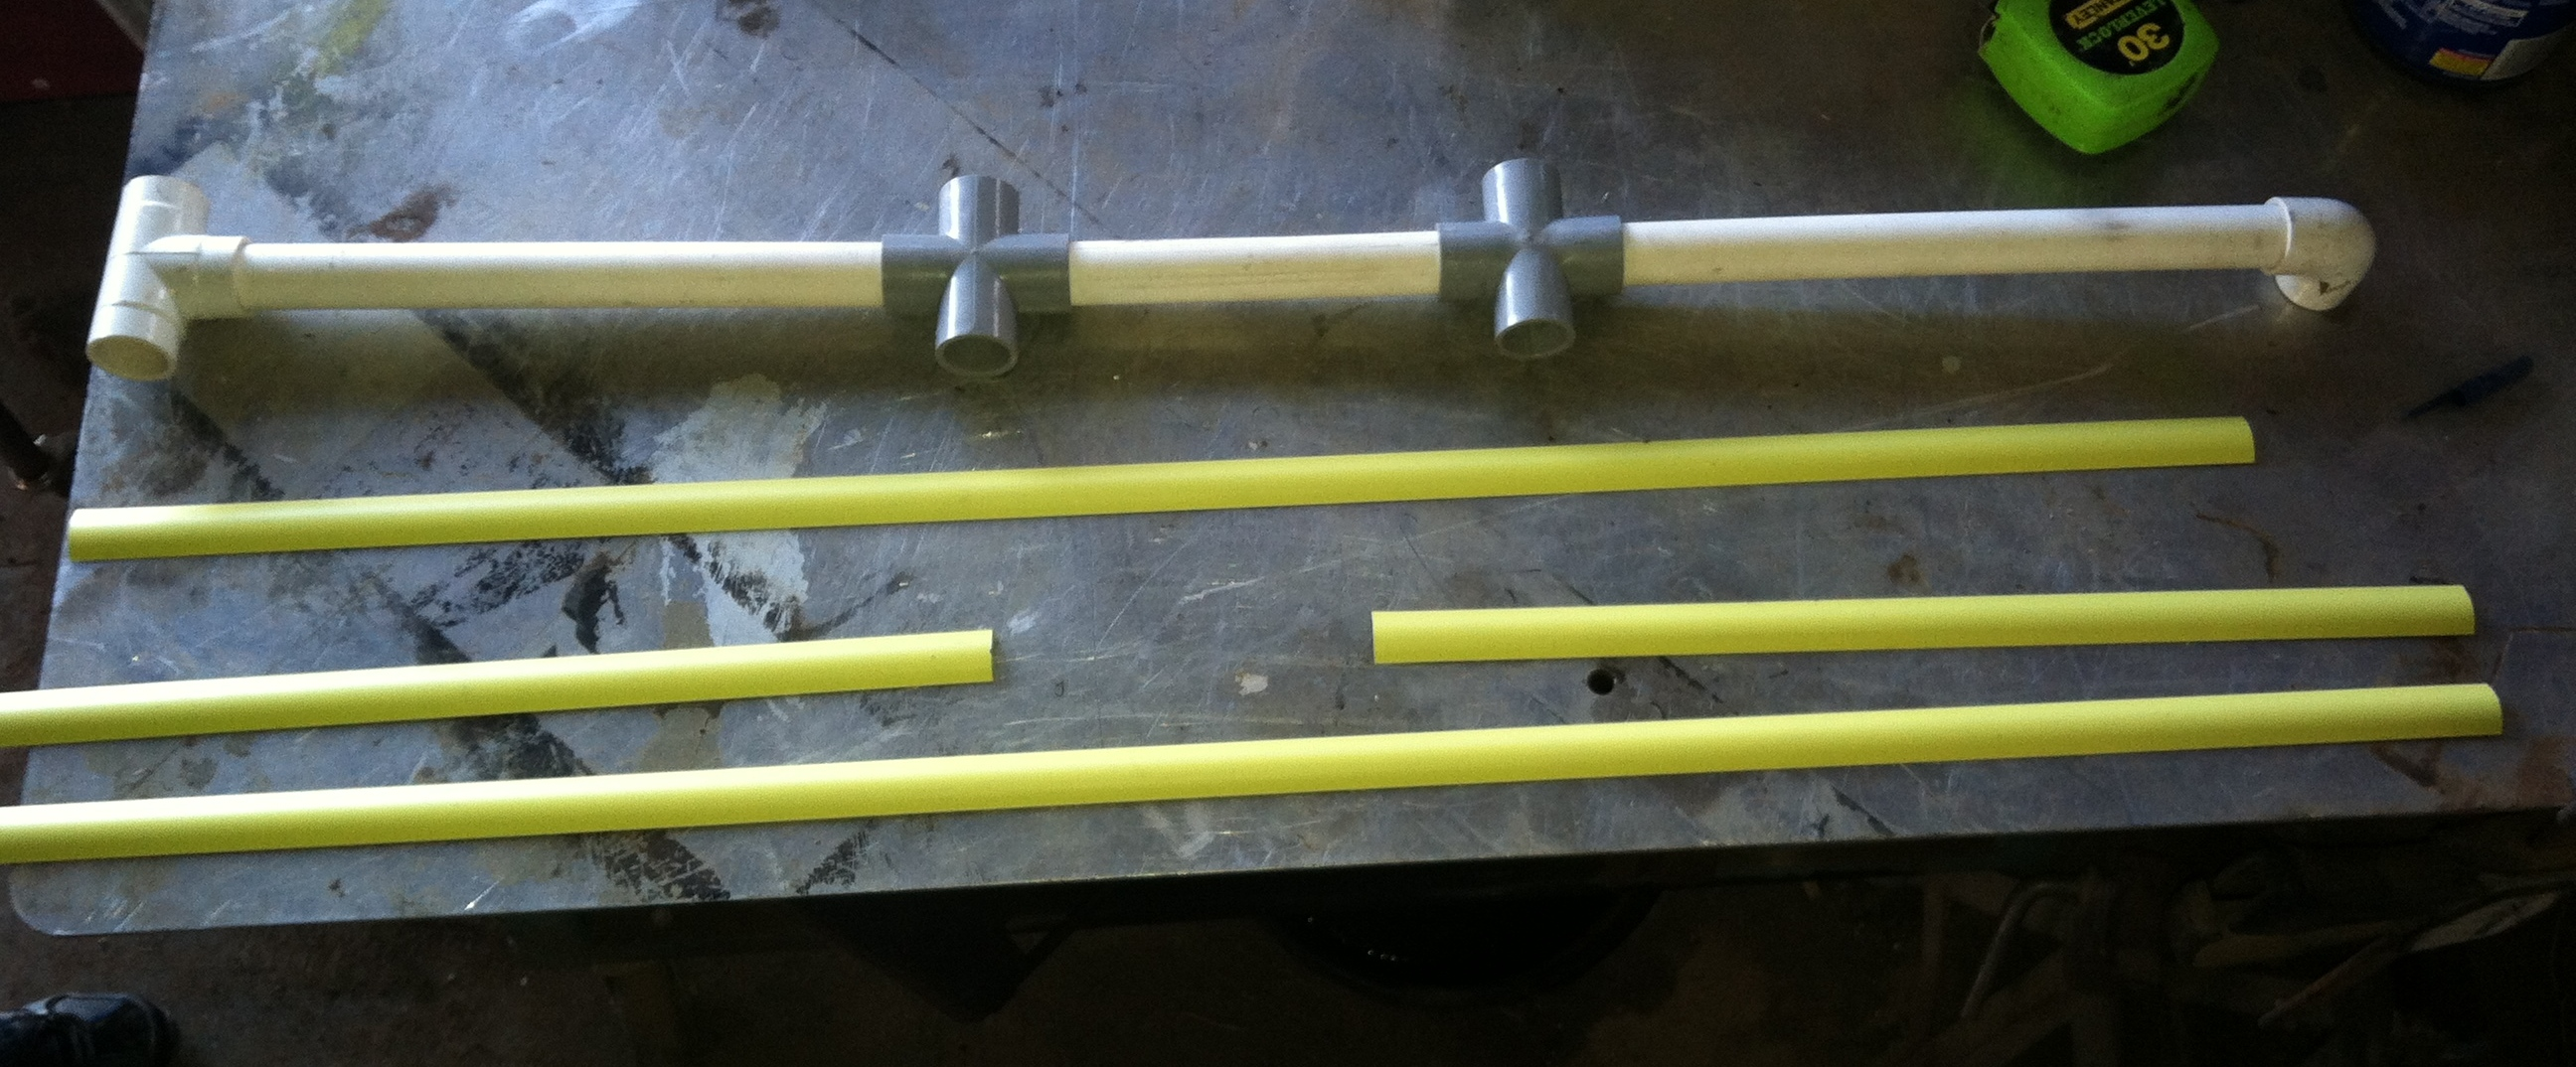
\includegraphics[width=0.7\textwidth]{images/cutting-elements.jpg} % Image showing the cutting process
    \end{center}
\end{frame}

% Step 2: Installing the Elements
\begin{frame}
    \frametitle{Step 2: Installing the Elements}
    \begin{itemize}
        \item Attach the Director element using hose clamps.
        \item Install the driven elements, ensuring a 1-inch separation between them.
        \item Secure the Reflector element at the back of the antenna.
    \end{itemize}
\end{frame}

% Step 3: Soldering the Wires
\begin{frame}
    \frametitle{Step 3: Soldering the Wires}
    \begin{itemize}
        \item Tin the ends of the driven elements using solder.
        \item Solder the RG-58 cable: Inner wire to one driven element, outer to the other.
        \item Connect the two driven elements with a 5-inch wire.
    \end{itemize}
    \begin{center}
        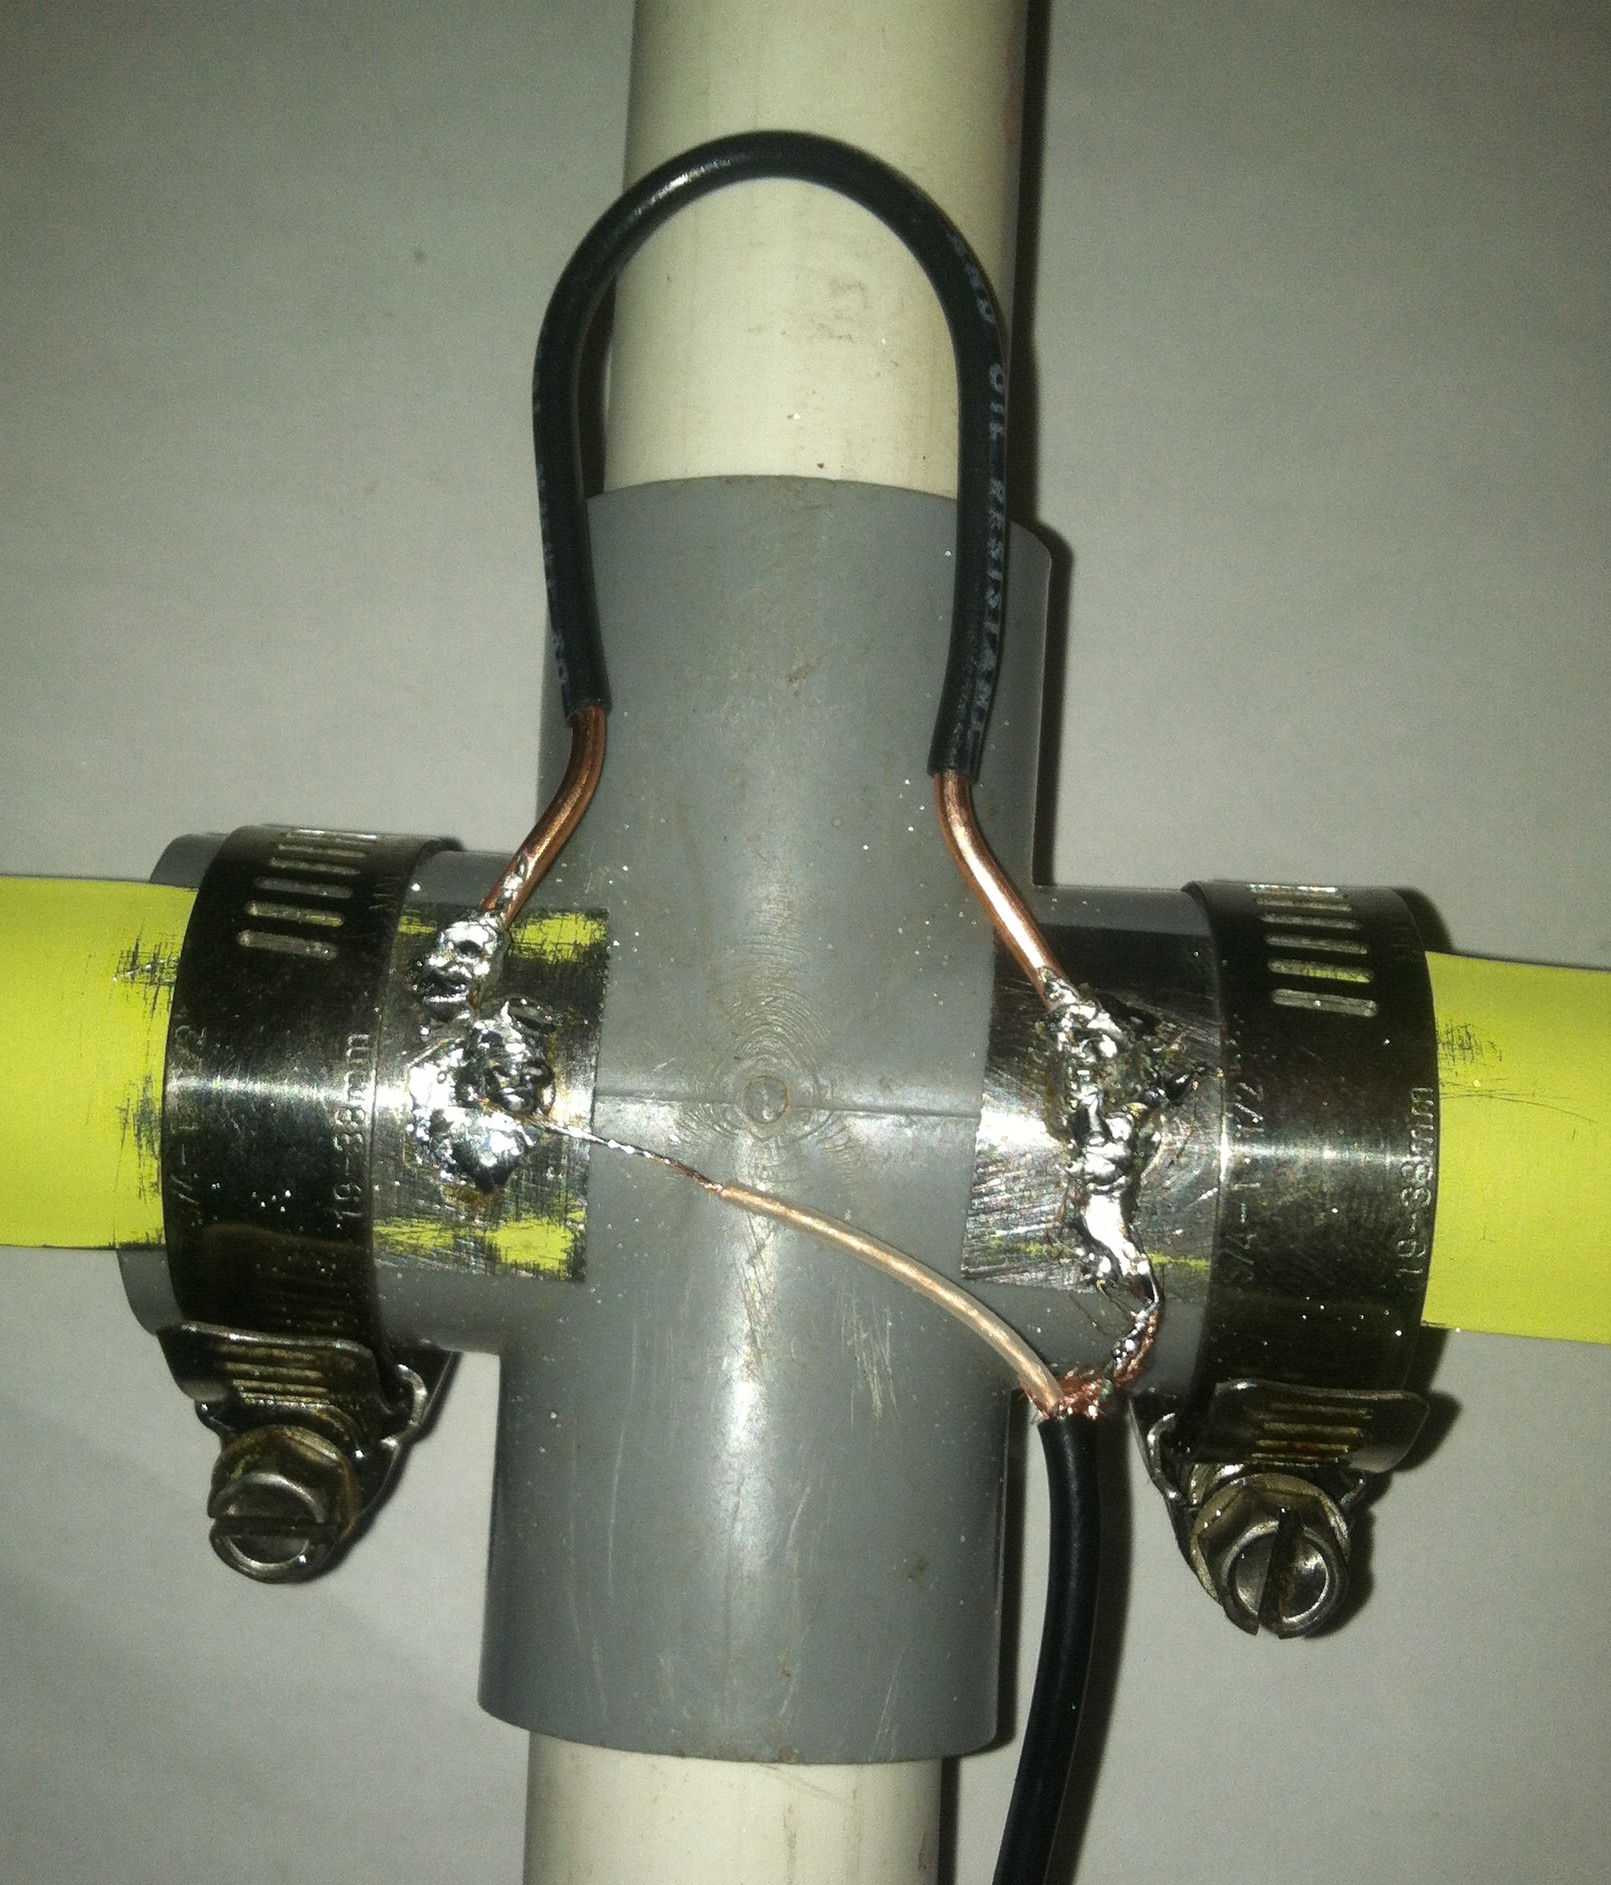
\includegraphics[width=0.4\textwidth]{images/soldering-1.jpg}
        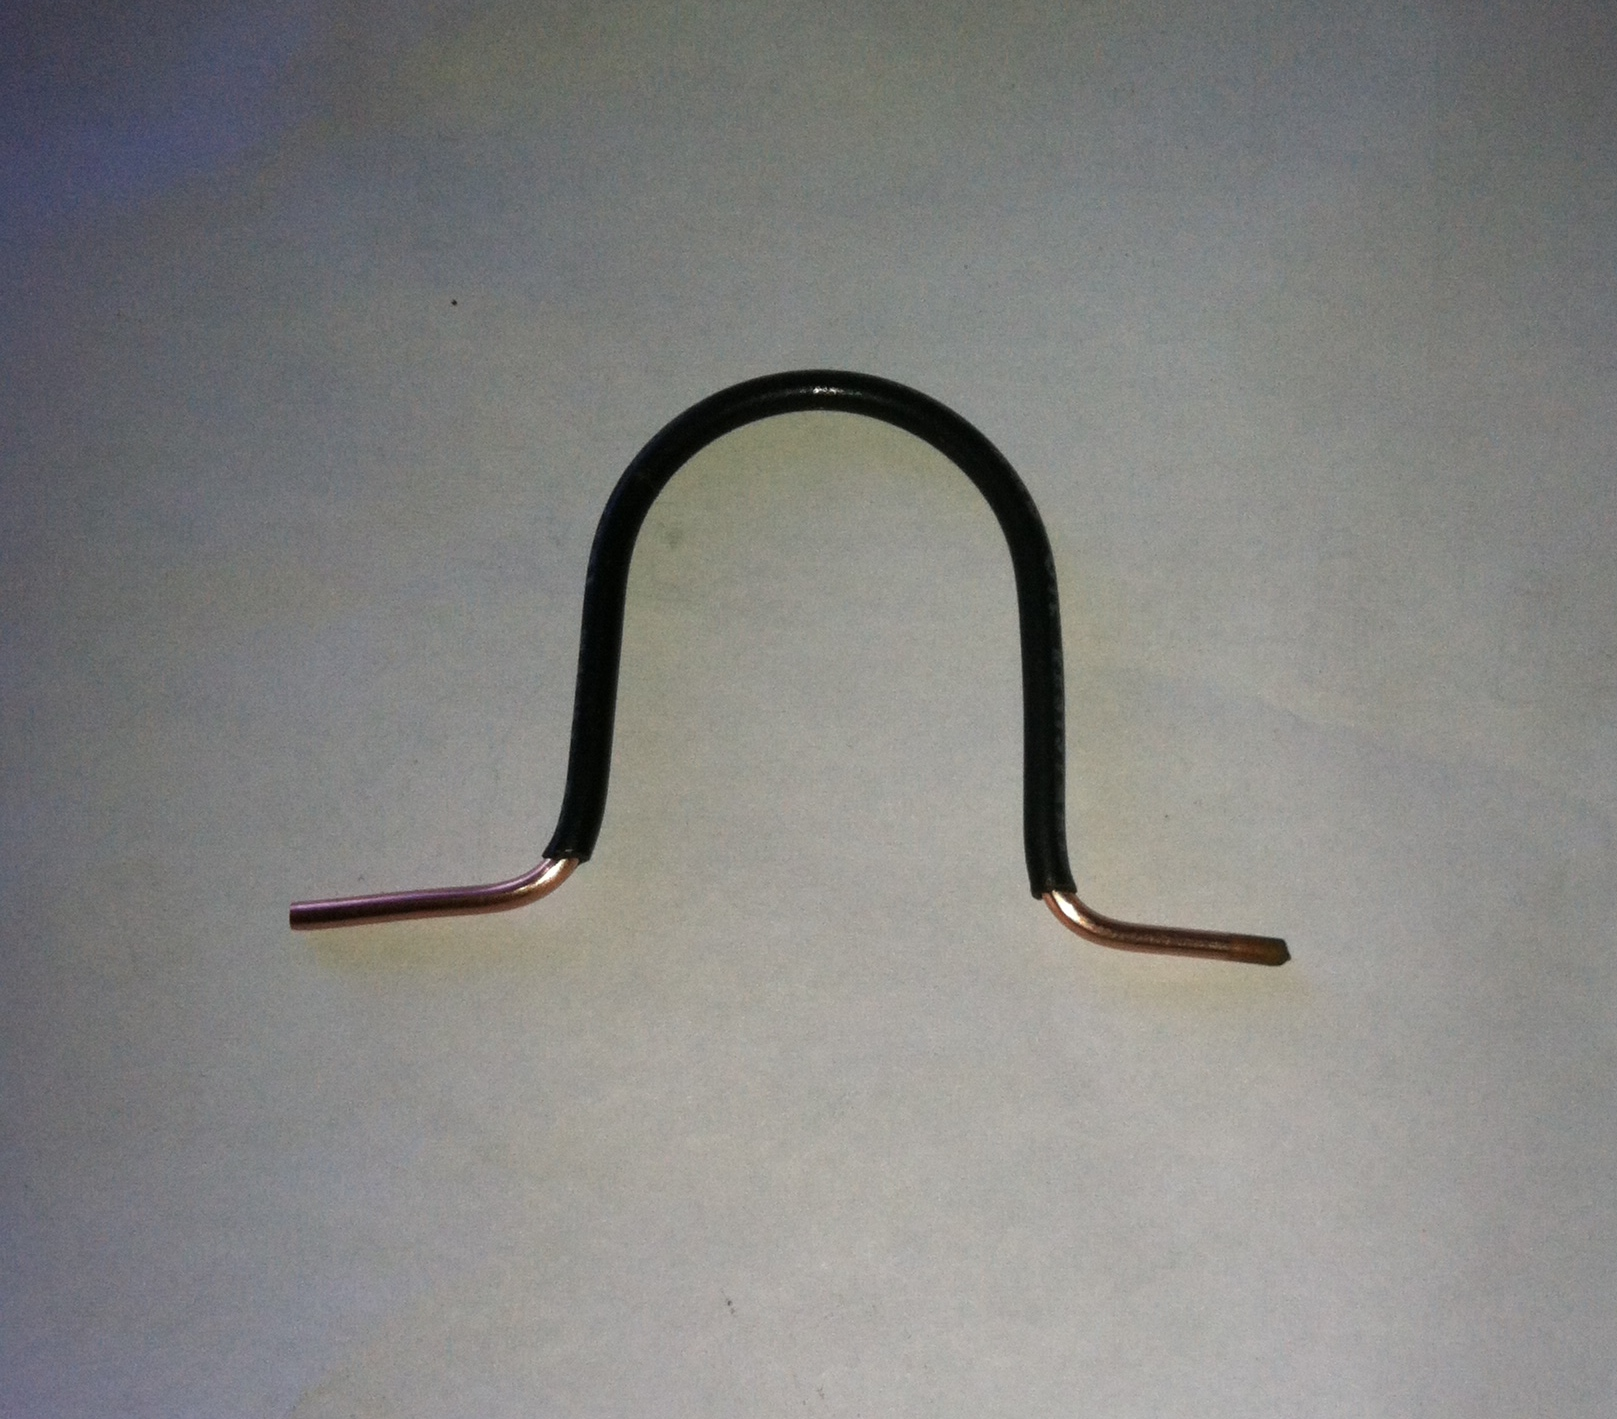
\includegraphics[width=0.4\textwidth]{images/soldering-2.jpg}
    \end{center}
\end{frame}

% Step 4: Adjusting the Antenna
\begin{frame}
    \frametitle{Antenna Adjustment} 
    \begin{itemize}
        \item Use an SWR meter to adjust the antenna.
        \item Fine-tune the driven elements if the SWR reading is higher than 1.2:1.
        \item Ensure the radio is powered off while making adjustments.
    \end{itemize}
\end{frame}

% -----------------------------------------------------------------------------
% Contact Us Slide
% Provides contact information for the workshop team and Wireless Club
% -----------------------------------------------------------------------------
\begin{frame}
    \frametitle{Contact Us}
    \begin{itemize}
        \item Questions? Feel free to contact us!
        \item Workshop Team Emails: \\
        \{\href{mailto:elarbi.m@northeastern.edu}{elarbi.m}, 
        \href{mailto:aviedov.v@northeastern.edu}{aviedov.v}, 
        \href{mailto:heaney.ma@northeastern.edu}{heaney.ma}\}[at]northeastern[d0t]edu
        \item General Workshop Email: \href{mailto:workshops@nuwireless.org}{workshops}[at]nuwireless[d0t]org
        \item Website: \url{https://nuwireless.org/}
        \item Location: Hayden Hall, Room 503
    \end{itemize}
    \vspace{1cm}
    \begin{flushright}
        \footnotesize{© 2024 Northeastern Wireless Club} \\
        \footnotesize{Design: \href{https://melarbi.com}{Muhammad Elarbi}, based on LaTeX Beamer}
    \end{flushright}
\end{frame}

% -----------------------------------------------------------------------------
% References Slide
% Lists all external resources used in the presentation
% -----------------------------------------------------------------------------
\section{References} 
\begin{frame} 
    \frametitle{References} 
    \begin{itemize} 
        \item Original design by Joe Leggio, WB2HOL (\url{http://theleggios.net/wb2hol/projects/rdf/tape_bm.htm}) 
        \item Additional designs: KC0TKS (\url{http://www.kc0tks.org}) and NT1K (\url{http://nt1k.com}) 
        \item This workshop is based on jcoman’s project tutorial on Instructables (\url{https://www.instructables.com/The-Tape-Measure-Antenna/}).
        \item All images used are sourced from jcoman’s tutorial on Instructables.
    \end{itemize}
\end{frame}

\end{document}
